\documentclass{article}
\usepackage{graphicx}
\begin{document}



\includegraphics[height=2.in]{images/test.png}   % compile using pdflatex
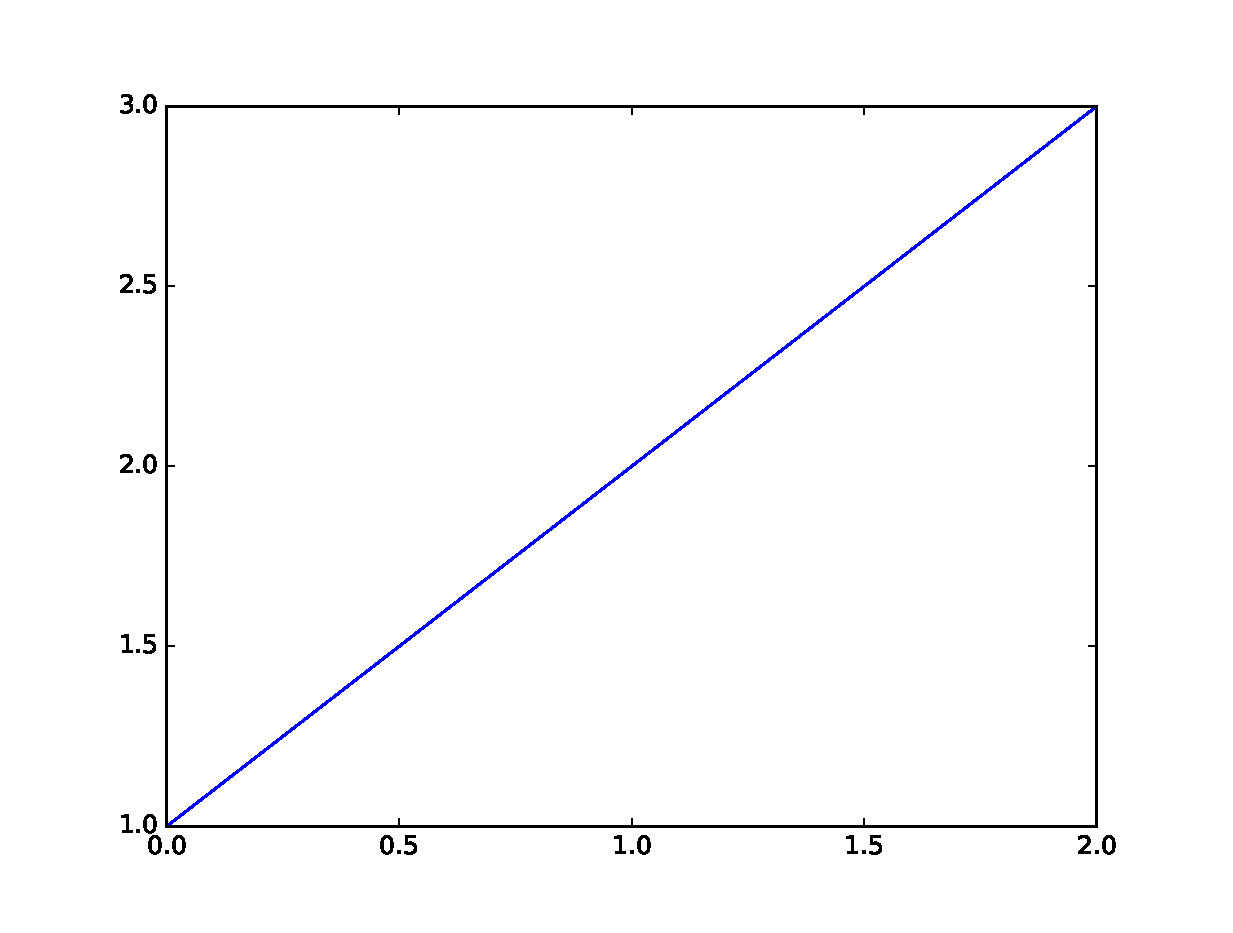
\includegraphics[height=2.in]{images/test.eps}   % compile using pdflatex
%\includegraphics[height=2.in]{images/test.ps}   % compile using latex
\end{document}

% pdflatex a.tex || latex a.tex

% use latex command for ps file
% latex a.tex; dvipdf a.dvi; bibtex a; latex a.tex; latex a.tex; rm -f a.aux; rm -f a.bbl; rm -f a.blg; rm -f a.log; rm -f a.out; rm -f *.bak && xdg-open a.pdf

% use pdflatex command for eps,png etc files
% pdflatex a.tex; bibtex a; pdflatex a.tex; pdflatex a.tex; rm -f a.aux; rm -f a.bbl; rm -f a.blg; rm -f a.log; rm -f a.out; rm -f *.bak && xdg-open a.pdf

% raster/bitmap graphics are composed of pixels e.g. created from photoshop
% while vector graphics are composed of paths or formulas e.g created
% from adobe illustrator.

% raster images: jpg, gif, png, tif, bmp, psd, eps and pdfs originating
% from raster programs e.g. Photoshop & Paint Shop, GIMP

% vector images: ai, cdr, svg, and eps & pdfs originating from vector
% programs e.g. CorelDraw, Inkscape

% 72 ppi or dpi for monitor display, webpage
% 300 ppi or dpi for printing


% jpg = small, no transparent background
% use = rectangle or square photos and photographs on your website.

% png = transparent background and is generally higher quality
% use = use = logos, icons and other images where a transparent background is preferred.

% gif = few solid colors and don’t have gradients
% use = simple web graphics such as web buttons, charts and icons.

% tif = larger and no loss in quality, not good for web since larger size
% use = use = images and photographs for high quality print.

% eps = An EPS file is a vector file of a graphic, text or illustration
% use = use = master logo files and graphics and print designs.

% ai = An AI file is a proprietary, vector file type created by Adobe
% use = creating logos, graphics, illustrations.

% (latex -interaction nonstopmode -halt-on-error -file-line-error a.tex && dvipdf a.dvi; bibtex a ; latex -interaction nonstopmode -halt-on-error -file-line-error a.tex ; latex -interaction nonstopmode -halt-on-error -file-line-error a.tex ) || (pdflatex a.tex ; bibtex a ; pdflatex a.tex ; pdflatex a.tex ); rm -f a.aux ; rm -f a.bbl ; rm -f a.blg ; rm -f a.log ; rm -f a.out ; rm -f *.bak ; rm -r a.dvi ; find . -name *eps-converted* -type f -exec rm -r {} + ; xdg-open a.pdf


% (latex -interaction nonstopmode -halt-on-error -file-line-error %e.tex && dvipdf %e.dvi; bibtex %e ; latex -interaction nonstopmode -halt-on-error -file-line-error %e.tex ; latex -interaction nonstopmode -halt-on-error -file-line-error %e.tex ) || (pdflatex %e.tex ; bibtex %e ; pdflatex %e.tex ; pdflatex %e.tex ); rm -f %e.aux ; rm -f %e.bbl ; rm -f %e.blg ; rm -f %e.log ; rm -f %e.out ; rm -f *.bak ; rm -r %e.dvi ; find . -name *eps-converted* -type f -exec rm -r {} + ; xdg-open %e.pdf

